\documentclass{standalone}
\usepackage{pgfplots}
\pgfplotsset{compat=newest}
\begin{document}
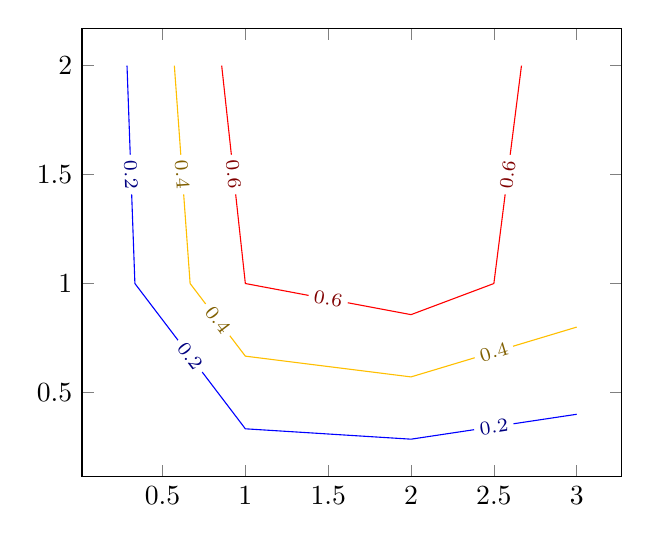
\begin{tikzpicture}
	\begin{axis}
	\addplot[contour prepared,
		contour prepared format=matlab]
	table {
% (0.2,5) ==> contour `0.2' (x), 5 points follow (y):
	   2.0000000e-01   5.0000000e+00 
	   3.0000000e+00   4.0000000e-01 
	   2.0000000e+00   2.8571429e-01 
	   1.0000000e+00   3.3333333e-01 
	   3.3333333e-01   1.0000000e+00 
	   2.8571429e-01   2.0000000e+00 
% (0.4,5) ==> contour `0.4', consists of 5 points
	   4.0000000e-01   5.0000000e+00 
	   3.0000000e+00   8.0000000e-01 
	   2.0000000e+00   5.7142857e-01 
	   1.0000000e+00   6.6666667e-01 
	   6.6666667e-01   1.0000000e+00 
	   5.7142857e-01   2.0000000e+00 
% (0.6,6) ==> contour `0.6', has 6 points
	   6.0000000e-01   6.0000000e+00 
	   2.6666667e+00   2.0000000e+00 
	   2.5000000e+00   1.0000000e+00 
	   2.0000000e+00   8.5714286e-01 
	   1.0000000e+00   1.0000000e+00 
	   1.0000000e+00   1.0000000e+00 
	   8.5714286e-01   2.0000000e+00 
		};
	\end{axis}
\end{tikzpicture}
\end{document}
